\documentclass[12pt]{report}

\usepackage{graphicx}
\usepackage{listings}
\usepackage{titlesec}
\usepackage{amsmath}
\usepackage{url}
\usepackage{biblatex}
\usepackage[hidelinks]{hyperref}
\usepackage{float}
\usepackage{subcaption}
\usepackage{geometry}

\geometry{
    left=20mm,
    right=20mm,
    top=20mm,
    bottom=20mm,
}

\addbibresource{references.bib}

\titleformat{\chapter}[display]
  {\normalfont\huge\bfseries}{\chaptertitlename\ \thechapter}{20pt}{\Huge}

\renewcommand{\chaptername}{Task}

\usepackage{inconsolata}

\lstset{
    basicstyle=\ttfamily,
    language=Python,
    frame=lines,
    literate={-}{-}1,
    breaklines=true,
}

\title{ID2090 A5}
\author{Anton Beny M S, ME23B015}
\date{May 2024}
\begin{document}

\maketitle
\newpage

\tableofcontents

\newpage

\chapter{Transform your chances}

\section{Introduction}
This task required us to perform convolution on two given functions using the Fourier transforms and output the final convolved function.

\section{Theory}

\subsection{Convolution}

The convolution \cite{enwiki:Convolution} of two functions $f_1, f_2$ is given by:

$$f_1 \ast f_2 = \int_{-\infty}^{\infty} f_1(k) f_2(x-k) dk$$

\subsection{Fourier Transform}

The Fourier transform \cite{enwiki:Fourier} of a function $f(x)$ is given by:

$$\mathcal{F}\{f\}(k) = \int_{-\infty}^{\infty} f(x) e^{-2\pi i k x} dx$$

\subsection{The Convolution Theorem}

The convolution theorem \cite{enwiki:Convolution_Theorem} states that the Fourier transform of the convolution of two functions is equal to the point-wise product of the Fourier transforms of the functions. Mathematically,

$$\mathcal{F}\{f_1 \ast f_2\}(k) = \mathcal{F}\{f_1\}(k) \cdot \mathcal{F}\{f_2\}(k)$$

In simpler terms, we can say that the convolution of two functions $f_1, f_2$ is given by:

$$f_1 \ast f_2 = \mathcal{F}^{-1} \{\mathcal{F}\{f_1\}\cdot\mathcal{F}\{f_2\}\}$$

\section{Code}

\subsection{Reading the functions}
The first step was to read the functions from the given file. The functions were given in latex form. I converted them to sympy expressions using the \texttt{latex2sympy2} module.

\begin{lstlisting}[caption={Reading the functions}]
from latex2sympy2 import latex2sympy as l2s

with open(sys.argv[1], "r") as file:
    f1, f2 = (l2s(line) for line in file.readlines())
\end{lstlisting}

The functions $f_1, f_2$ are:

\begin{figure}[H]
    \centering
    \begin{subfigure}{0.45\textwidth}
        \centering
        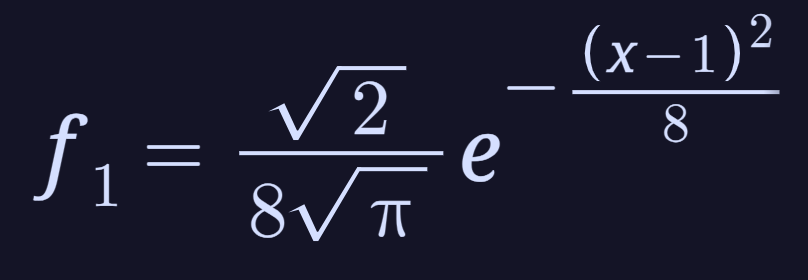
\includegraphics[width=\linewidth]{f1.png}
        \caption{$f_1$}
        \label{fig:f1}
    \end{subfigure}
    \begin{subfigure}{0.45\textwidth}
        \centering
        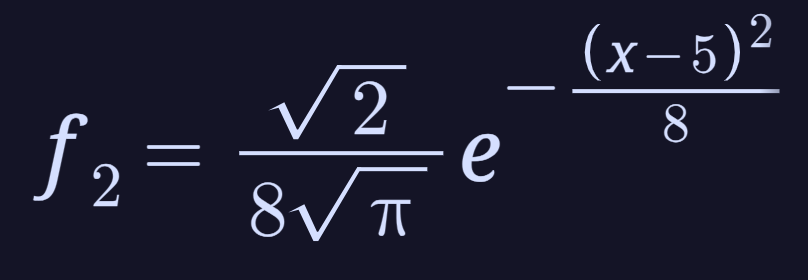
\includegraphics[width=\linewidth]{f2.png}
        \caption{$f_2$}
        \label{fig:f2}
    \end{subfigure}
    \caption{Functions $f_1$ and $f_2$}
    \label{fig:f1_f2}
\end{figure}

\subsection{Fourier Transform}
The next step was to find the Fourier transforms of the functions $f_1, f_2$. This was done using the \texttt{sympy} module, which has in-built functions for Fourier Transforms.

\begin{lstlisting}[caption={Finding the Fourier transforms of the functions}]
x, k = sp.symbols("x k")

F1 = sp.fourier_transform(f1, x, k)
F2 = sp.fourier_transform(f2, x, k)
\end{lstlisting}

The values of F1 and F2 are:

\begin{figure}[H]
    \centering
    \begin{subfigure}{0.45\textwidth}
        \centering
        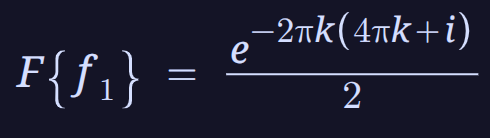
\includegraphics[width=\linewidth]{F1.png}
        \caption{$\mathcal{F}\{f_1\}$}
        \label{fig:F1}
    \end{subfigure}
    \begin{subfigure}{0.45\textwidth}
        \centering
        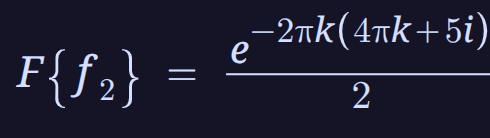
\includegraphics[width=\linewidth]{F2.png}
        \caption{$\mathcal{F}\{f_2\}$}
        \label{fig:F2}
    \end{subfigure}
    \caption{Fourier Transforms of $f_1$ and $f_2$}
\end{figure}

\subsection{Convolution}
Finally, the convolution of the two functions was found by taking the inverse Fourier transform of the product of the Fourier transforms of the functions.

\begin{lstlisting}[caption={Finding the Convolution}]
F = sp.inverse_fourier_transform(F1 * F2, k, x)
\end{lstlisting}

The final convolved function is:

\begin{figure}[H]
    \centering
    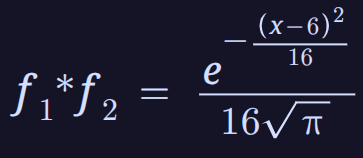
\includegraphics[width=0.5\linewidth]{F.png}
    \caption{Convolved function $f_1 \ast f_2$}
    \label{fig:F}
\end{figure}

\section{Observations}

Here are a few things that I observed, while working on the Task

\begin{itemize}
    \item The \texttt{sympy} has a lot of in-built functions that made it very easy to perform the Fourier Transforms and Inverse Fourier Transforms.
    \item While researching, I found that \texttt{sympy} has an in-built function for Convolution as well. However, that is only for discrete convolution, and not for continuous convolution.
    \item To compare the performance of convolution using Fourier Transforms vs traditional convolution, I implemented the traditional convolution as well. The implementation is shown below:

          \begin{lstlisting}
F = sp.integrate(f1.subs(x, k) * f2.subs(x, x - k), (k, -sp.oo, sp.oo))
        \end{lstlisting}
          I used the time interval of execution to compare the two methods. The Fourier Transform method had an average execution time of \textbf{0.913} seconds, while the traditional convolution method had an average execution time of \textbf{0.312}. I believe that the traditional convolution method is faster because it doesn't involve any complex mathematical operations such as Fourier Transforms, but rather just a simple integral.
    \item Graphically, the functions $f_1, f_2$ and their convolved function look as shown below:

          \begin{figure}[H]
              \centering
              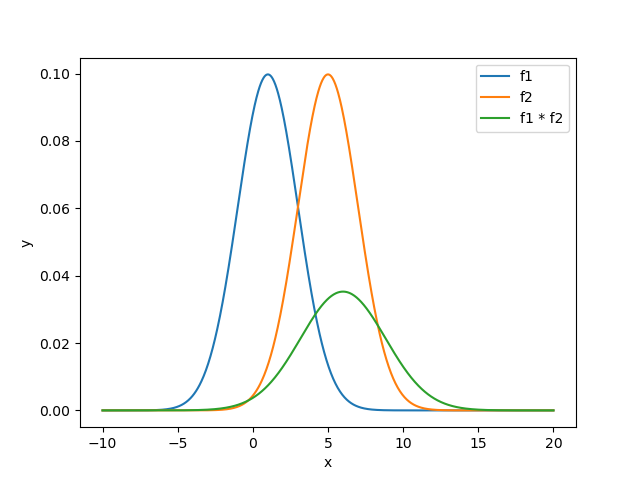
\includegraphics{Figure_1.png}
              \caption{Graphs of $f_1, f_2, f_1 \ast f_2$}
          \end{figure}
    \item In the example above, the functions $f_1, f_2$ are gaussian functions. We can observe that the convolved function is also a gaussian function. This shows that the convolution of two gaussian functions is also a gaussian function.
\end{itemize}

\section{Conclusion}

\begin{itemize}
    \item This was a very interesting task. I learnt the basics of Fourier Transforms and Convolution and the relationship between them.
    \item \texttt{sympy} made this task pretty easy to implement. It allowed me to easily convert the latex functions to sympy expressions and do the necessary mathematical operations.
\end{itemize}

\newpage

\chapter{Poised for Poiseuille flow}

\section{Introduction}

In this task, we are required to solve the Navier-Stokes equation \cite{enwiki:Navier-Stokes}. The problem is simplified using the following assumptions:

\begin{itemize}
    \item Incompressible flow ($\rho$ is constant) $\implies \partial \rho = 0$
    \item Fully Developed Flow (z-velocity not dependent on z) $\implies \frac{\partial v_z}{z} = 0$
    \item $\theta$ - symmetric flow ($\theta$ components and their changes can be neglected) $\implies v_\theta = 0$
    \item Impenetrable wall (Zero radial velocity at a radius equal to pipe radius) $\implies v_r(r=R) = 0$
    \item Continuous and Smooth (Differentiable) flow profile.
\end{itemize}

\section{Theory}

\subsection{Navier-Stokes Equation}

Beginning with the general form of the Navier-Stokes equation:

$$\frac{\partial\rho}{\partial t} + \frac{1}{r}\frac{\partial(\rho r v_r)}{\partial\rho} + \frac{\partial(\rho v_z)}{\partial z} + \frac{1}{r} \frac{\rho v_\theta}{\partial\theta} = 0$$

We can simplify this equation using the assumptions given above to get:

$$\frac{1}{r}\frac{\partial(\rho r v_r)}{\partial\rho} = 0$$
$$r v_r = \text{constant}$$
$$v_r = \frac{c}{r}$$

At $r = $0, $v_r$ is finite. Therefore, $c = 0$ and $v_r = 0$.

Using this, we can now assume that $\vec{v} = v_z \hat{e}_z$. The equation now becomes:

$$\frac{\partial(\rho \vec{v})}{\partial t} + (\vec{v} \cdot \nabla) \vec{v} = \rho\vec{g} - \nabla P + \mu \nabla^2\vec{v}$$

This is simplified to:

$$\frac{\partial P}{\partial z}= \mu \nabla^2v_z$$

$$\frac{\partial P}{\partial z} = \mu (\frac{\partial^2 v_z}{\partial r^2} + \frac{1}{r} \frac{\partial v_z}{\partial r})$$

From product rule, we get that:

$$\frac{1}{r}\frac{\partial(r \frac{\partial v_z}{\partial r})}{\partial r} = \mu (\frac{\partial^2 v_z}{\partial r^2} + \frac{1}{r} \frac{\partial v_z}{\partial r})$$

The final equation to solve is:

$$\frac{\partial P}{\partial z} = \frac{1}{r}\frac{\partial(r \frac{\partial v_z}{\partial r})}{\partial r}$$

To solve this equation:

$$\frac{\partial P}{\partial z} r \partial r = \partial(r \frac{\partial v_z}{\partial r})$$

Integrating both sides, we get:

$$\frac{\partial P}{\partial z} \frac{r^2}{2} = r \frac{\partial v_z}{\partial r} + C_2$$

$$\frac{\partial P}{\partial z} \frac{r}{2} \partial r = \partial v_z + \frac{C_2}{r} \partial r$$

Integrating once again, we get:

$$v_z = C_1 + C_2\cdot \text{log(r)} + \frac{(\frac{\partial P}{\partial z}) r^2}{4}$$

The differential equation can also be solved using the \texttt{sp.dsolve} function in \texttt{sympy}, to get the same result.

The boundary conditions are:

\begin{itemize}
    \item $v_z(0) \neq \pm \infty$
    \item $v_z(R) = 0$
\end{itemize}

Applying the boundary conditions, we get:

$$v_z = \frac{1}{4}\frac{\partial P}{\partial z}(r^2 - 1)$$

\section{Code}

\subsection{Reading the function}
The first step was to read the given function and convert it from latex to a sympy expression.

\begin{lstlisting}[caption={Reading the function}]
import sympy as sp
from latex2sympy2 import latex2sympy as l2s

with open(sys.argv[1], "r") as file:
    P = l2s(file.readline())
\end{lstlisting}

\subsection{Solving the equation}
To solve the Navier-Stokes equation, I used \texttt{sp.dsolve} function, which solves the given differential equation.

$$\nabla P = \frac{\mu}{r}\frac{\partial(r \frac{\partial v_z}{\partial r})}{\partial r}$$

\begin{lstlisting}[caption={Solving the equation}]
navier_stokes = sp.Eq(
    sp.Derivative(rho * vz, z) + vz * sp.Derivative(vz, z),
    rho * gz
    - sp.Derivative(P, z)
    + mu * (sp.Derivative((r * sp.Derivative(vz, r)), r)) / r,
)

solution = sp.dsolve(navier_stokes, vz)
\end{lstlisting}
The general solution obtained from the \texttt{sp.dsolve} function is:

$$v_z = C_1 + C_2\cdot \text{log(r)} + \frac{(\nabla P) r^2}{4}$$

\subsection{Applying the boundary conditions}
The boundary conditions are applied to the general solution to get the final solution.

\begin{lstlisting}[caption={Applying the boundary conditions}]
general_solution = solution.rhs
C1, C2 = sp.symbols("C1 C2")

boundary_conditions = [
    sp.Eq(general_solution.subs(r, 0), C1),
    sp.Eq(general_solution.subs(r, R), 0),
]

constants = sp.solve(boundary_conditions, (C1, C2))
particular_solution = general_solution.subs(constants)

assumptions = {
    "g_z": 0,
    "mu": 1,
    "R": 1,
}

final_solution = particular_solution.subs(assumptions)
\end{lstlisting}

\subsection{Generating the .cpp file}
Finally, the solution is writen to a .cpp file using the \texttt{sp.ccode} function, which converts the sympy expression to a C++ expression. I assumed that the executable's name is \texttt{vel.out}.

\begin{lstlisting}
print(
    """#include <iostream>
#include <cmath>
int main(int argc, char *argv[]) {{
    double r = std::stod(argv[1]);
    std::cout << std::abs({}) << "\\n";
}}""".format(
        str(sp.ccode(final_solution))
    ),
    file=open("vel.cpp", "w"),
)

import subprocess

subprocess.run(["g++", "-O2", "vel.cpp", "-o", "vel.out"])
\end{lstlisting}
\section{Observations}
\begin{itemize}
    \item The Navier-Stokes equation is a very complex equation to solve. The assumptions used in this task simplified the equation to a great extent.
    \item Once again, the \texttt{sympy} module impressed me with its capabilities. It was able to solve the differential equations and also apply the boundary conditions to get the final solution. Moreover, it has an in-built function \texttt{sp.ccode} to convert the sympy expression to a C++ expression, which, I believe is pretty cool.
\end{itemize}
\section{Conclusion}

\begin{itemize}
    \item I learnt a lot about the Navier-Stokes equation and the basics of fluid dynamics through working on this task. Overall, it was another interesting task, and I especially liked it, when I found out about the \texttt{sp.ccode} function.
\end{itemize}

\printbibliography
\end{document}
